\section{Resolución por \textit{Programación Dinámica}}
	\subsection{Descripción del algorítmo}

	La solución por Programación Dinámica utiliza memoización: casos menores se guardan en una memoria interna y son reutilizados para calcular casos mayores.

	En el algoritmo que se propone, la memoria toma forma de arreglo de dos dimensiones, donde cada dimensión expresa la posición en la lista donde se encuentra el último elemento pintado de uno u otro color. Al calcular un casillero, se toma el color más avanzado y se recorren los anteriores para encontrar la mejor subsolución.

	Se debe considerar que no se calcula ninguno de los valores correspondientes a la diagonal de este arreglo, es decir, posiciones que representarían que un mismo elemento está pintado de ambos colores, ya que esto no es válido.

	\begin{algorithm}[H]
		\NoCaptionOfAlgo
		
		\KwData{Lista, la lista de números a pintar}

		\KwData{Memoria, el arreglo de dos dimensiones con soluciones previas}

		\KwData{Rojo, la posición del rojo que estamos calculando ahora}

		\KwData{Azul, la posición del azul que estamos calculando ahora}

		\If{Memoria[Rojo][Azul] no fue calculado todavía}{
			\uIf{Rojo == Azul == $|Lista|$}{
				Estamos en el caso base (nada pintado)

				Guardamos en Memoria[Rojo][Azul] |Lista| (todos sin pintar) y lo marcamos como calculado
			}
			\uElseIf{Azul == $|Lista|$ \textbf{or} Rojo $>$ Azul}{
				Buscamos el mejor valor para los rojos anteriores.

				\For{i $\leftarrow$ 0 \KwTo Rojo - 1}{
					\If{i $\neq$ Azul \textbf{and} Lista[i] < Lista[Rojo]}{
						Llamada recursiva: \{Lista, Memoria, i, Azul\}
					}
				}

				Llamadas recursiva: \{Lista, Memoria, $|Lista|$, Azul\} (caso sin pintar rojos)

				Sea Min el menor resultado de todas las llamadas recursivas que realizamos

				Guardamos en Memoria[Rojo][Azul] Min - 1 (fue pintado Rojo) y lo marcamos como calculado
			}
			\Else{
				Buscamos el mejor valor para los azules anteriores.

				\For{i $\leftarrow$ 0 \KwTo Azul - 1}{
					\If{i $\neq$ Rojo \textbf{and} Lista[i] > Lista[Azul]}{
						Llamada recursiva: \{Lista, Memoria, Rojo, i\}
					}
				}

				Llamada recursiva: \{Lista, Memoria, Rojo, $|Lista|$\} (caso sin pintar azules)

				Sea Min el menor resultado de todas las llamadas recursivas que realizamos

				Guardamos en Memoria[Rojo][Azul] Min - 1 (fue pintado Azul) y lo marcamos como calculado
			}
		}

		\KwResult{Memoria[Rojo][Azul], la mejor subsolución con Rojo y Azul como últimos elementos pintados de cada color (se garantiza que esa memoria fue calculada)}
	\end{algorithm}

	En la implementación provista, la memoria se rellena de forma \textit{bottom-up}, es decir los casos más básicos primero, pero el orden no altera el producto ya que en cada paso la llamada recursiva asegura que cualquier posición que se necesite esté calculada, y solo se calcula una vez.

	A su vez, cada dimensión de la memoria tiene de un casillero de largo extra para considerar el caso en que no se han pintado todavía casilleros de ese color. La memoria almacena si ya fue calculada y el mejor resultado posible para la misma.

	\subsection{Cota de complejidad}

	Este algoritmo realiza, en peor caso, n llamadas recursivas por paso. Sin embargo, como cada resultado se memoiza, cada llamada recursiva cuesta O(1) amortizado.

	Como el algoritmo rellena toda la memoria (salvo las posiciones inválidas), y el tamaño de la misma es de $n^2$ (siendo n el largo de la lista), el orden de complejidad del algoritmo es $O(n^3)$.

	\pagebreak
	\subsection{Gráfico de complejidad}

	El siguiente gráfico, si bien fue medido de la misma manera que los otros, utiliza una escala en microsegundos. Tanto la forma de la figura, más gradual que en los gráficos anteriores, como la necesidad de usar una unidad de medida más precisa dejan en claro que este algoritmo es mucho más eficiente.

	\begin{center}
	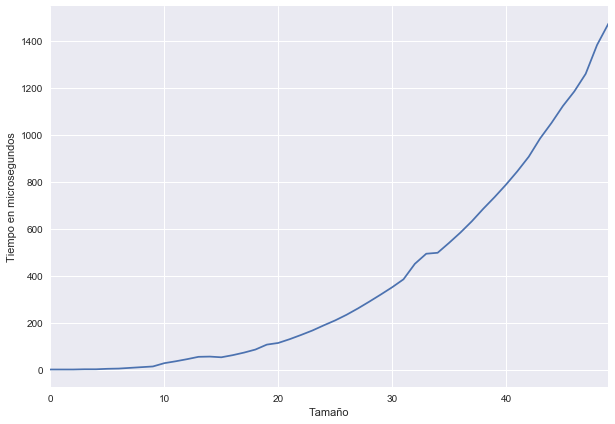
\includegraphics[width=.8\textwidth]{ej3.png}
	\end{center}

	A modo de comparación se agrega también el siguiente gráfico en el que se muestran los tres algoritmos utilizando la escala logarítmica, y utilizando nuevamente segundos para el eje Y.

	En este caso se puede notar la diferencia en orden de complejidad comparado con los algoritmos basados en Backtracking: mientras que aquellos se asemejan levemente a una recta lineal en escala logarítmica (por su complejidad exponencial), este algoritmo es polinómico y por ende describe una curva logarítmica.

	\begin{center}
	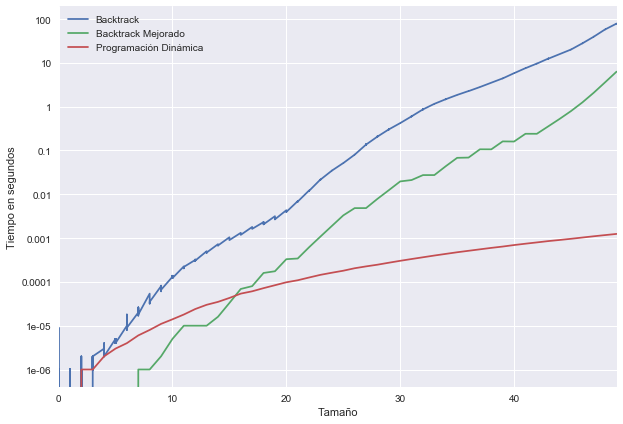
\includegraphics[width=.8\textwidth]{ej3-2.png}
	\end{center}